\documentclass[a4paper,10pt,bibtotoc]{scrartcl}
\usepackage{a4wide,usg}
\usepackage{draftcopy}

%% Do NOT remove: required to extract SVN information
\svnInfo $Id$

%% Adjust page footer
\fancyfoot[LE,LO]{LOFAR-USG-ICD-004: Radio Sky Image Cubes}
\fancyfoot[RE,RO]{\textsc{lofar} Project}

\begin{document}

%%_______________________________________________________________________________
%% Titlepage

\title{LOFAR Data Format ICD \\ Radio Sky Image Cubes \\
{\normalsize Document ID: LOFAR-USG-ICD-004} \\
{\normalsize Version 2.07.05} \\
{\normalsize SVN Repository Revision: \svnInfoRevision}}
\author{L.~B\"ahren, K.~Anderson, J.~Masters}
\date{\small{SVN Date: \svnInfoDate}}
\maketitle

\tableofcontents

\clearpage

%%_______________________________________________________________________________
%% Change record of the document

\section*{Change record}
\addcontentsline{toc}{section}{Change record}

\begin{center}
  %% Table head
  \tablefirsthead{
    \hline
    \sc Version & \sc Date & \sc Sections & \sc Description of changes \\
    \hline
  }
  \tablehead{
    \multicolumn{4}{r}{\small\sl continued from previous page} \\
    \hline
    \sc Version & \sc Date & \sc Sections & \sc Description of changes \\
    \hline
  }
  %% Table tail
  \tabletail{
    \hline
    \multicolumn{4}{r}{\small\sl continued on next page} \\
  }
  \tablelasttail{\hline}
  %% Table contents
  \begin{supertabular}{lllp{9.5cm}}
    \shrinkheight{-3em}

    0.0  & 2009-04-03 & All & Initial revision \\

    0.1  & 2009-05-07 & All & Further full revision, new format \\

    0.2  & 2009-06-04 & \ref{sec:context and motivation},
    \ref{sec:organization of the data} & Revision on A2 comments \\

    0.3  & 2009-06-17 & All, + \ref{sec:coordinates group} & Full revision,
    migration to \LaTeX \\

    0.4  & 2009-06-23 & \ref{sec:coordinates group} & Revision of attributes \\

    0.5  & 2009-07-01 & All & Structural overhaul, all ICDs \\

    0.6  & 2009-07-20 & \ref{sec:organization of the data} \& \ref{sec:detailed
    structure} & Structural adjustment, Coordinate group. \\

    0.7  & 2009-07-27 & \ref{sec:organization of the data}, \ref{sec:detailed
    structure} \& App. & Document redisposition, Filename, Glossary appendix \\

    0.8  & 2009-09-22 & All & Recast group naming conventions, consistency \\

    0.9  & 2009-09-23 & \ref{sec:coordinates group} & Added missing coordinate
    type, added comments \\

    0.10 & 2009-09-29 &\ref{sec:detailed structure} & Cleaning up of
    coordinate group attributes \\

    0.11 & 2009-12-12 & \ref{sec:detailed structure} & Moved coordinates group
    table to external file \\

    0.12 & 2010-01-08 & \ref{sec:detailed structure} & Refactor LOFAR group
    type table \\

    0.13 & 2010-04-19 & \ref{sec:detailed structure} & Refactor Sec.~4.1
    $\Rightarrow$ 4.1.1, 4.1.2 \\

    0.14 & 2010-04-28 & \ref{sec:common lofar attributes} & New HBA naming
    convention (change in CLA)\\

    0.15 & 2010-05-03 & \ref{sec:common lofar attributes} & New
    \verb|ANTENNA_SET| values, vis-a-vis \verb|HBA| modes.\\

    0.16 & 2010-06-04 & Appendix & Removed section ``Coordinate group examples''
    from the appendix; detailed description and examples now can be found in
    \texttt{LOFAR-USG-ICD-002} \cite{lofar.icd.002} \\

    2.00.00 & 2010-07-08 & Cover & Changed `revision' to `version';  updated
    this version number to 2.00.00 for LOFAR ICDs 1 through 7 to put them on the same
    version numbering scheme.\\

    2.01.00 & 2010-10-20 & \ref{sec:source table} & Rewrite of the source table
    definition, as this was never fleshed out properly; description now also in
    sync with LOFAR-USG-ICD-008 \cite{lofar.icd.008}. Tracking of open question
    in the appropriate section of the document. \\

    2.01.01 & 2010-12-06 & All & Using \LaTeX\ package \texttt{hyperref} for
    references, enabling better navigation through the document and access to
    external resources. Added note on version numbering scheme. \\

    2.02.00 & 2011-01-05 & \ref{sec:organization of the data} \&
    \ref{sec:detailed structure} & Major cleanup, diagram revision.  Reset
    \verb|GROUPTYPE| value examples in coordinates to read as
    \verb|<CoordType>Coord|, eg., \verb|`StokesCoord'|.  This convention had
    not been observed in some locations.  See further comment at
    \ref{sec:coordinates group} , `The Coordinates Group.'\\

    2.02.10 & 2011-01-05 & \ref{sec:coordinates group} & revamp file
    group to match diagram, other tweaks. \\

    2.02.11 & 2011-01-25 & \ref{sec:image group} & Adjustment of attribute names
    to be more consistent; added labels and captions to tables and figures. \\

    2.03.00 & 2011-02-01 & \ref{sec:overview} & move and insert image table,
    descr. text \\

    2.03.01 & 2011-03-10 & All & Maintain list of references
    through Bib\LaTeX\ database. \\

    2.04.00 & 2011-03-30 & All & Storage of source model parameters; Update of
    figures; Trimmed down number of coordinate sections. \\

    2.05.00 & 2011-04-27 & \ref{sec:image dataset} & Attributes describing shape
    of data array \\

    2.05.01 & 2011-05-11 & \ref{sec:coordinates group} & Added paragraph with
    notation conventions \\

    2.05.02 & 2011-05-24 & \ref{sec:introduction} \& \ref{sec:overview} & Cleaning
    up text, adjusting references. \\

    2.05.03 & 2011-05-25 & All & Addressing some of the comments provided by
    J.~Swinbank. \\

    2.06.00 & 2011-05-25 & All & Removing \textsl{Average Images Groups} from
    the data structures tree; this does not add anything new, but rather confuses
    the overall architecture of the data file. Removed section ``Interfaces'',
    which was not being used anyway. \\

    2.06.01 & 2011-05-26 & \ref{sec:common lofar attributes} & Removed figure
    with antenna array configurations. \\

    2.06.02 & 2011-06-09 & All & Started addressing some of the
    comments from common reading of the ICD by the Data Formats Group. \\

    2.06.03 & 2011-06-21 & All & Second round addressing some of the
    comments from common reading of the ICD by the Data Formats Group. \\

    2.06.04 & 2011-06-29 & All & Matching up group type attributes and notation. \\

    2.06.05 & 2011-07-06 & All & Matching up group type attributes and
    notation; consolidation of labels to refer to standard sections
    and tables. \\

    2.07.00 & 2011-09-28 & All & Cleaning up attributes attached to the
    source table. Add new group \verb|PSF_INFO| as element to image group. \\

    2.07.01 & 2011-10-05 & \ref{sec:open-questions} & Remove oustanding issue
    which was closed by 2.07.00. Tweak formatting \& fix typos. \\

    2.07.02 & 2011-10-05 & \ref{sec:open-questions} & Add note on system log
    group to open questions. \\

    2.07.03 & 2011-12-19 & \ref{sec:detailed structure} & Include standard
    introduction to metadata. \\

    2.07.04 & 2011-12-19 &  & Add standard data types description. \\

    2.07.05 & 2012-03-06 & cover   & Added draftcopy package for background 'draft' text.\\

\end{supertabular}
\end{center}

\input version_numbering

\input types

\input notation

\subsection*{Acknowledgements}

The document was originally developed by K.~Anderson in collaboration
with J.~Masters.

\clearpage

%% _______________________________________________________________________________
%% Introduction

\section{Introduction}
\label{sec:introduction}

\subsection{Purpose and Scope}
\label{sec:purpose and scope}

The natural interface between the standard pipelines and the science pipelines
is a well-defined set of standard LOFAR data products. These products are the
outputs of the pipelines which run on Central Processing facility
(CEP) and are the natural starting points for the science pipelines.

We note that any or all of these standard data products may also be
accompanied by various ancillary data or ``metadata''. Metadata might
include information such as instrument health, configuration or
performance, gain curves, flagging tables, etc. In some cases this
information may simply take the form of pointers to entries in the
calibration database via header keywords. Alternatively, metadata may
also be packaged in the same file with the main data in the form of
additional tables or extensions.

This \icd{} sets forth a formal data interface specification for the
LOFAR data products refered to as ``\textbf{Radio Sky Image Cube}'' and is
intended to be the formal interface control agreement between the
LOFAR project, observers/users of LOFAR data products, and the
eventual LOFAR science archive facility.

\subsection{Context and Motivation}
\label{sec:context and motivation}

A LOFAR \textbf{Radio Sky Image Cube} will be the data hosting structure for
sky image data produced by LOFAR, irrespective of their scientific purpose.
It is one of the tasks of the LOFAR project to define and describe the
structure of the LOFAR \textbf{Radio Sky Image Cube} format.

While image hypercubes are the primary data product of the imaging
pipeline, they are accompanied by a number of by-products, such as
flagging information, CLEAN components, local and global sky models
(LSM, GSM), etc. In the more traditional approach, where all such
products are stored and managed separately, a large amount of
book-keeping is required to maintain consistency. For the LOFAR
project, a \textbf{Radio Sky Image Cube} product will be defined within the context
of the Hierarchical Data Format 5, or HDF5 \cite{hdf5}. HDF5 allows
for storage, not only of the data, but for the associated and related
meta-data describing the image cube contents, conditions of
observations, etc.. As an ``all-in-one'' wrapper, the HDF5 format
simplifies the management of what are expected to be very large
datasets that formats such as FITS cannot pragmatically accommodate.

There has been much discussion of a putative need for LOFAR
\textbf{Radio Sky Image Cube} headers to adhere to FITS-like header
keywords. Though it is envisioned that the LOFAR project will provide observers and other
users with FITS format image files upon request, it is not entirely
necessary that HDF5 header keywords match FITS keyword conventions in
a LOFAR Sky Image file itself. A format conversion layer can
certainly be developed to provide rigorous transformation of LOFAR
headers into more restricted FITS header keyword sets. However,
development of such a layer would be simplified in the event that
LOFAR Sky Image files make use of \textit{de facto} FITS standard
keywords as much as possible.

For the purposes of further discussion regarding Sky Image file
adherence to FITS keyword standards, the \textsl{ESO Data Interface
 Control Document} \cite{eso.dic}, has been adopted as the FITS
keyword model.

\begin{comment}
  Is this really true? \cite{eso.dic} not only uses FITS notation, but
  actually defines the data products in terms of FITS files.
\end{comment}

\input applicable_documents

%% ______________________________________________________________________________
%%                                                              Section: Overview

\section{Overview}
\label{sec:overview}

LOFAR imaging data will be presented in a number of LOFAR data formats, all of
which will provide data arrays of differing dimensions, depending upon the
respective observation. Sky Image Cubes, Rotation Measure Cubes, Near-Field
Cosmic Ray Images, etc., all have different dimensions and coordinate types.
Table~\ref{tab:lofar_data_types} illustrates the various image data array
dimensions that LOFAR imaging may produce.

\input coordinates_image_table

Each data type is described in detail by an appropriate interface
control document. This document pertains to, and describes only those
data conforming to the LOFAR datatype ``Radio Sky Image''.

The remainder of this document is structured as follows:
Sec.~\ref{sec:organization of the data} will present a high-level view of the
hierarchical structure of LOFAR data files, file form, and semantic
conventions the interface will adhere to, including a statement of the
primary data product format, HDF5. These conventions will also include
names, meaning, and physical units that may be used to generate and
interpret the data files. Sec.~\ref{sec:detailed structure} will
present the low-level specification for the data, including a
description of the structure of LOFAR Sky Image files, and the various
group entities and sub-structures comprising these image data files,
i.e. LOFAR group types, units, physical quantities.

%% _______________________________________________________________________________
%% Organization of the data

\section{Organization of the data}
\label{sec:organization of the data}

\subsection{High level LOFAR Sky Image file structure}

A LOFAR \textbf{Radio Sky Image Cube} (a hypercube image file) will be defined
within the context of the the Hierarchical Data Format, version 5
(HDF5). In an effort to minimize the hierarchical depth of the file
structure, a Sky Image file is designed to be as ``flat'' as possible,
providing access to the necessary data without undue hierarchical tree
crawling.

Therefore, the Sky Image HDF5 file structure will comprise a primary
group, a ``root group'' in HDF5 nomenclature, which may be considered
equivalent to a primary header/data unit (HDU) of a standard
multi-extension FITS file. This primary group will consist only of
header keywords (Attributes in HDF5 nomenclature) describing general
properties of an observation, along with pointers to contained
subgroups. These subgroups will comprise an arbitray number of
``Image groups'' (see Sec.~\ref{sec:image group}), where an Image
group will contain data and meta-data for a single sub-band of an
observation.

\subsection{Overview of Sky Image Groups}
\label{sec:overview of sky image groups}

A LOFAR \textbf{Radio Sky Image Cube} will then comprise \texttt{System Log Group}
just below the root level which contains logs and parameter files
which are relevant to the entire file. Additionally, just below the
root level, the Sky Image file will contain an arbitrary,
observation-dependent number of \texttt{Image Groups} containing a
\texttt{Coordinates Group}, a \texttt{Source Group}, and a
\texttt{Processing History Group}, which contains pertinent logs and
parameter sets of the relevent image sub-band.

These main building blocks of the Sky Image HDF5 file are (also see
Fig.~\ref{fig:top-level view} below):

\begin{enumerate} \parskip 0pt
\item \textbf{File Root Group} (\verb|ROOT|). The root level of the file contains
  the majority of associated meta-data, describing the circumstances
  of the observation. These data attributes include time, frequency
  and other important characteristics of the dataset. See
  Sec.~\ref{sec:root group} for a detailed description.

\item \textbf{System Logs Group} (\verb|SYS_LOG|). This is a catch-all
  envelop encapsulating information about all the system-wide steps of
  processing which are relevant to the entire observation, such as
  parameter sets and processing logs. See Sec.~\ref{sec:sylog group}
  for a detailed description.

\item \textbf{Image Groups} (\verb|IMAGE_{NNN}|). Each observation
  sub-band image is stored as a seperate group within the file,
  containing its own set of four (4) sub-groups. Characteristics
  about each sub-band image are stored as Attributes in group headers.
  LOFAR imaging can produce up to 244 sub-band images, which will be
  the maximum number of image groups possible in a LOFAR Sky Image.
  Each Image group will contain one Data group, which will in turn
  contain one dataset as an ndarray, along with associated
  attributes. See Sec.~\ref{sec:image group} for a detailed description.

\item \textbf{Source Table} (\verb|SOURCE_TABLE|). Each observation
  sub-band processing produces a file describing what is called the
  Local Sky Model (LSM). A \textbf{Source Table} will contain a
  table of the sources listed in a processing file, a \verb|.skymodel| file.
  Attributes will describe the columnar data. See Sec.~\ref{sec:source
    table} for a detailed description.

\item \textbf{Coordinates Groups} (\verb|COORDINATES|). Each
  \texttt{Image Group} contains one \texttt{Coordinates Group}, which
  stores the relevant world coordinate conversions.

\item \textbf{Processing History Groups} (\verb|PROCESS_HISTORY|)
  can be found on the \texttt{Image Group} level. These are catch-all
  envelops encapsulating information about all the steps of
  processing, such as parameter sets and processing logs. See
  Sec.~\ref{sec:processing history group} for a detailed description.

\item \textbf{Data Group/Image Data arrays} (\verb|DATA|). For each Image Group, the
  subband image data are stored as ndarrays in the respective Data
  group -- it is at this 4th hierarchical depth where the image data
  reside.
\end{enumerate}

\subsection{Hierarchical structure of the Sky Image file}
\label{sec:hierarchical structure}

A LOFAR \textbf{Radio Sky Image Cube} will then comprise an arbitrary,
observation-dependent number of these Image groups.

\begin{figure}[htbp]
 \centering
 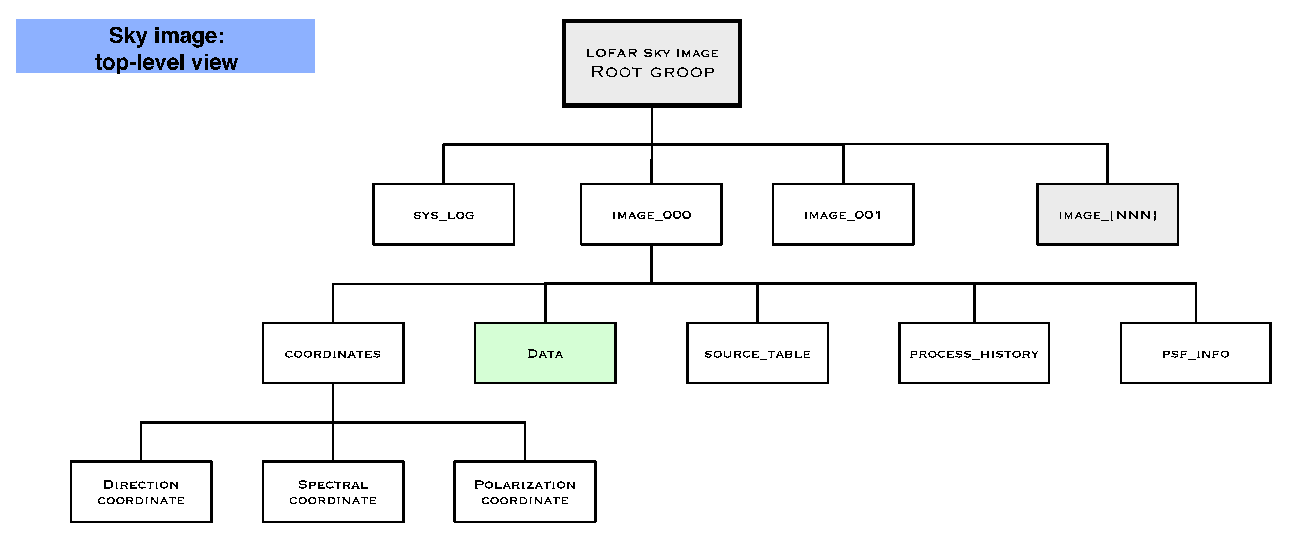
\includegraphics[width=\textwidth]{figures/Sky_TopLevelView.eps}
 \caption{Top-level view on the structure of a sky image.}
 \label{fig:top-level view}
\end{figure}

This structure can be represented through HDF5 as a \textsc{posix}-style hierarchy:

\begin{lstlisting}
OBS_NUMBER/SYS_LOG
OBS_NUMBER/IMAGE_000
OBS_NUMBER/IMAGE_000/COORDINATES
OBS_NUMBER/IMAGE_000/COORDINATES/COORDINATE_0
OBS_NUMBER/IMAGE_000/COORDINATES/COORDINATE_1
OBS_NUMBER/IMAGE_000/COORDINATES/COORDINATE_2
OBS_NUMBER/IMAGE_000/IMAGE_DATA
OBS_NUMBER/IMAGE_000/SOURCE_TABLE
OBS_NUMBER/IMAGE_000/PSF_INFO
OBS_NUMBER/IMAGE_000/PROCESS_HISTORY
OBS_NUMBER/IMAGE_001
OBS_NUMBER/IMAGE_001/COORDINATES
OBS_NUMBER/IMAGE_001/COORDINATES/COORDINATE_0
OBS_NUMBER/IMAGE_001/COORDINATES/COORDINATE_1
OBS_NUMBER/IMAGE_001/COORDINATES/COORDINATE_2
OBS_NUMBER/IMAGE_001/IMAGE_DATA
OBS_NUMBER/IMAGE_001/SOURCE_TABLE
OBS_NUMBER/IMAGE_001/PSF_INFO
OBS_NUMBER/IMAGE_001/PROCESS_HISTORY
...
\end{lstlisting}

Similarly, one can represent the same structure as such:

\begin{lstlisting}
L1002977_sky.h5              ...  (Root) Group
|-- SYS_LOG                  ...  Group
|-- IMAGE_000                ...  Group
|   |-- COORDINATES          ...  Group
|   |   |-- COORDINATE_0     ...  Group
|   |   |-- COORDINATE_1     ...  Group
|   |   `-- COORDINATE_2     ...  Group
|   |-- IMAGE_DATA           ...  Dataset
|   |-- SOURCE_TABLE         ...  Dataset
|   |-- PSF_INFO             ...  Group
|   `-- PROCESS_HISTORY      ...  Group
|-- IMAGE_001                ...  Group
|
`-- IMAGE{NNN}               ...  Group
\end{lstlisting}

%% _______________________________________________________________________________
%%                                            Section: Detailed Data Specification

\section{Detailed Data Specification}
\label{sec:detailed structure}

\input metadata_intro

\subsection{The Root Group ({\tt ROOT})}
\label{sec:root group}

The LOFAR file hierarchy begins with the top level \textbf{File Root
  Group} (\verb|ROOT|). This is the file entry point for the data, and
the file node by which navigation of the data is provided.  The
\textbf{File Root Group} will comprise a set of attributes that describe
the underlying file structure, observational metadata, the LOFAR Radio Sky Image
data, as well as providing hooks to all groups attached to the
\textbf{File Root Group}.

This section will specify two sets of attributes that will appear in
the \textbf{File Root Group} of all LOFAR data product files: a set of
\cla\ (CLA) that will be common to all LOFAR science
data products, and a set of attributes that are specific to LOFAR Sky
Image data.  Though these attributes will all appear together in the
\texttt{Root} attribute set, they are separated in this document in
order to demarcate those general LOFAR attributes that are applicable
across all data, and those attributes that are image-specific. In
other words,
\begin{verse}
  \verb|Root Attributes = Common LOFAR Attributes + Additional Root Group Attributes.|
\end{verse}
The {\cla} are the first attributes of any LOFAR \textbf{File Root Group}.

\subsubsection{\cla}
\label{sec:common lofar attributes}

This section will specify a set of attributes that will be common to
LOFAR science data products.  These ``\cla'' will
appear as attributes at the root level of all LOFAR data files.
\textit{All} LOFAR data products, including Sky Images \textit{inter
  alia,} will share a common set of metadata root-level attributes.
These \cla\ are to be the first set of attributes of
any LOFAR file root group.

Table~\ref{tab:lofar common metadata} lists the {\cla} (CLA) which can
be found in all LOFAR data file types. These attributes are required
to be in the Root Group; if a value is not available for an
attributes, a \verb|`NULL'| maybe used in its place.

\input lofar_common_metadata

\begin{table}[htbp]
  \centering
  \begin{tabular}{|lrp{6cm}|}
    \hline
    \sc \textbf{General LOFAR Group} & \sc \textbf{Value} & \textbf{Description} \\
    \hline
    Root           & \verb|`Root'|   & Top-level LOFAR group type \\
    System Log     & \verb|`SysLog'| & System log files, parsets \\
    \textbf{Image} & \verb|`Image'|  & Image group \\
    \hline \hline
    \sc \textbf{Image Group Subgroups} & \textbf{Value} & \textbf{Description} \\
    \hline
    Data group (\verb|DATA|)   & \verb|`Data'| & This is a Sky Image dataset. \\
    Source table (\verb|SOURCE_TABLE|) & \verb|`SourceTable'| & This is a Source table. \\
    Processing History group &\verb|`ProcessHistory'| & This is a
    Processing History group \\
    % Masks group & \verb|`Masks'| & This is a Masks group \\
    \hline
    \hline
    \sc \textbf{Coordinate Groups} & \textbf{Value} & \textbf{Description} \\
    \hline
    Coordinates Group        & \verb|`Coordinates'|
                             & This is a Coordinates group \\
    Direction coord group    & \verb|`DirectionCoord'|
                             & This is a direction coordinate group \\
    Spectral coord group     & \verb|`SpectralCoord'|
                             & This is a frequency coordinate group \\
    Polarisation coord group & \verb|`PolarisationCoord'|
                             & This is a polarisation coordinate group \\
    \hline
  \end{tabular}
  \caption{LOFAR Sky Image Group Types}
  \label{tab:group types}
\end{table}

\subsubsection{Additional Sky Image Root Attributes}
\label{sec:additional root group attributes}

As explained at the begin of Sec.~\ref{sec:root group} above, the root group of
a \textbf{Radio Sky Image Cube} will contain a set of attributes, which can
be broken down into two subsets: 1) a set of \cla\ (CLA) that will be common to all
LOFAR science data products, and 2) a set of attributes that are specific to LOFAR
Sky Image data. With the {\cla} already listed in Sec.~\ref{sec:common lofar attributes}
above, this section will focus on the second subset of root
group attributes, as they are specific to a \textbf{Radio Sky Image Cube}.

This root group header will comprise general information about the
observation itself, sparing relevant data details for the headers of
the lower order sub-groups.  Table~\ref{tab:attributes root group}
presents additional root group attributes for a LOFAR \textbf{Radio Sky Image Cube}
that do not appear in the {\cla} table.\footnote{\textbf{ *} Indicates attributes that may
  \textit{migrate from the root group} and be broadcast to individual
  \texttt{Image} groups.  Recent observations have indicated that
  different sub-bands potentially can have different integration
  times.}

\begin{table}[htbp]
  \centering
  \begin{tabular}{|lrp{10cm}|}
    \hline
    \textsc{Field/Keyword} & \textsc{Type} & \sc Description \\
    \hline \hline
    \small\verb|INPUT_DATA| & \texttt{string} & Descriptor to
    track the input data source, from which the image was created;
    this can be a visibility dataset, but as well streaming data
    (where no intermediate data product is being produced). \\
    \small\verb|NOF_IMAGES| & \small\verb|int| &
    \small{\texttt{N}} Image groups in this file \\
    \small\verb|TARGET_RA| & \small\verb|double| &
    \small\verb|RA| of \small\verb|TARGET| (at LOFAR core) \\
    \small\verb|TARGET_DEC| & \small\verb|double| &
    \small\verb|Dec| of \small\verb|TARGET| (at LOFAR core) \\
    \hline
  \end{tabular}
  \caption{Additional root group attributes specific to a Radio Sky Image Cube}
  \label{tab:attributes root group}
\end{table}

%%_______________________________________________________________________________
%% Subsection: The System Logs Group (SYS_LOG)

\input groups_sys_log

%%_______________________________________________________________________________
%% Subsection: The Image Group (IMAGE_NNN)

\subsection{The Image Group ({\tt IMAGE\_\{NNN\}})}
\label{sec:image group}

The \texttt{Image} group will be an HDF5 group serving as a container
for the four sub groups described below. An \texttt{Image} group is
designed to be as complete and self-contained an image cube as
possible, and will contain relevant data and metadata for a particular
processed sub-band of a LOFAR observation.  However, any breakout
protocol will be required to inherit some or all root group attributes
in order to function as a stand-alone image.  The adopted form allows
for relatively simple extraction and conversion in a FITS-compatible
form.

An \texttt{Image} group will comprise four sub groups. These four
groups, two hierarchical levels below the ``root group'' in a LOFAR Sky
Image (Fig.~\ref{fig:top-level view}), will be

\begin{itemize}
\item A \verb|COORDINATES| group that will contain one or more
  subgroups of kinds \texttt{LinearCoord, TabularCoord, SpectralCoord,
    DirectionCoord, StokesCoord}, that will describe various axes of
  the associated dataset.
\item A \verb|IMAGE_DATA| dataset that will contain a dataset array.
\item A \verb|SOURCE_TABLE| that will be a tabular representation of a
  Local Sky Model, as well as clean component used for the
  deconvolution of the image.
\item A \verb|PROCESS_HISTORY| group, which will be a meta-data container
  holding various processing products such as log files, parameter sets, RFI
  mitigation tables, etc.
\end{itemize}

The diagram below illustrates the form of an Image group in a LOFAR
Sky Image file.  The table of Image group attributes is notably sparse
here and the reader must bear in mind that the Coordinates groups will
contain most of the rest of the relevent Image group metadata
(\textit{see \ref{sec:coordinates group}, ``Coordinates group''})

\begin{lstlisting}
IMAGE_{NNN}
|-- GROUPTYPE                       ...  Attr.          string
|-- REFERENCE_FREQUENCY_VALUE       ...  Attr.          double
|-- REFERENCE_FREQUENCY_UNIT        ...  Attr.          string
|-- REFERENCE_BANDWIDTH_VALUE       ...  Attr.          double
|-- REFERENCE_BANDWIDTH_UNIT        ...  Attr.          string
|-- EFFECTIVE_FREQUENCY_VALUE       ...  Attr.          double
|-- EFFECTIVE_FREQUENCY_UNIT        ...  Attr.          string
|-- EFFECTIVE_BANDWIDTH_VALUE       ...  Attr.          double
|-- EFFECTIVE_BANDWIDTH_UNIT        ...  Attr.          string
|-- COORDINATES                     ...  Group
|   |-- COORDINATE_0                ...  Group
|   |-- COORDINATE_1                ...  Group
|   `-- COORDINATE_2                ...  Group
|-- IMAGE_DATA                      ...  Dataset
|-- SOURCE_TABLE                    ...  Dataset
`-- PROCESS_HISTORY                 ...  Group
\end{lstlisting}

\begin{table}[htbp]
  \centering
  \begin{tabular}{|llllp{6cm}|}
    \hline
    \sc Field/Keyword & \sc H5Type & \sc Type & Value &\sc Description \\
    \hline \hline
    \small\verb|GROUPTYPE| & Attr.
                           & \verb|string|
                           & \verb|`Image'|
                           & LOFAR group type \\
    \small\verb|REFERENCE_FREQUENCY_VALUE| & Attr.
                           & \verb|double|
                           & ---
                           & Numerical value of the reference frequency. \\
    \small\verb|REFERENCE_FREQUENCY_UNIT| & Attr.
                           & \verb|string|
                           & ---
                           & Physical unit of the reference frequency. \\
    \small\verb|REFERENCE_BANDWIDTH_VALUE| & Attr.
                           & \verb|double|
                           & ---
                           & Numerical value of the reference bandwidth. \\
    \small\verb|REFERENCE_BANDWIDTH_UNIT| & Attr.
                           & \verb|string|
                           & ---
                           & Physical unit of the reference bandwidth. \\
    \hline
    \small\verb|COORDINATES|     & Group   & --- & --- & Coordinates group         \\
    \small\verb|IMAGE_DATA|      & Dataset & --- & --- & Image dataset             \\
    \small\verb|SOURCE_TABLE|    & Dataset & --- & --- & Source list table/dataset \\
    \small\verb|PROCESS_HISTORY| & Group   & --- & --- & Processing history group  \\
    \hline
  \end{tabular}
  \caption{Components attached to the image group.}
  \label{tab:Image group Attributes}
\end{table}

%% _______________________________________________________________________________
%% Subsection: The Coordinates Group (COORDINATES)

\subsection{The Coordinates Group ({\tt COORDINATES})}
\label{sec:coordinates group}

Coordinate information within a LOFAR \textbf{Radio Sky Image Cube}
will exist in what is called a \textbf{Coordinates group}, which will
act as a container for a number of Coordinates group objects.
The \textbf{Coordinates group} (\verb|COORDINATES|) will be a subgroup
of an \textbf{Image group} container, and may contain one or more subgroups that will
describe relevent axes of the coordinates' associated \texttt{Data}
group using one or a combination of coordinate subgroups, where the
enumerated are Direction coordinate, Spectral coordinate and
Polarization coordinate.

\input coordinates_group_table
\input coordinates_frames_location

The attributes, as presented in Table \ref{tab:coordinates-group},  summarize the
overall characteristics of the set of coordinates collected within this group:
\begin{itemize}
\item \verb|GROUPTYPE| -- Identifier for the type of group, ``Coordinates''.
\item \verb|NOF_COORDINATES| -- The number of coordinate
  objects/groups contained within the coordinates group.
\item \verb|NOF_AXES| -- The number of coordinate axes associated with the
  coordinate objects. Keep in mind, that a coordinate can have multiple (coupled)
  axes:  e.g. a direction coordinate is composed of two axes.
\end{itemize}

The layout of the embedded sub-groups will depend on the type of coordinate, of
which there are several types.

\subsubsection{Direction coordinate}
\label{sec:coord-direction}

\input coordinates_coord_direction

\subsubsection{Spectral coordinate}
\label{sec:coord-spectral}

\input coordinates_coord_spectral

\subsubsection{Polarization coordinate}
\label{sec:coord-polarization}

\input coordinates_coord_polarization

%%_______________________________________________________________________________
%% Subsection: The Image Dataset (DATA)

\subsection{The Image Dataset ({\tt DATA})}
\label{sec:image dataset}

The \textbf{Image Dataset} is the object within the \textbf{Radio Sky Image Cube}
structure responsible for the actual storage of the image pixel
data. As such the dataset is a multi-dimensional array, storing
intensity values as function of direction on the sky
$(\mathrm{Lon},\mathrm{Lat})$, frequency ($\nu$) and polarization
component ($p$):

\begin{eqnarray}
  I & = & I (p,\nu,\mathrm{Lat},\mathrm{Lon})
\end{eqnarray}

The quantities attached to the array axes are described through the
coordinates group (Sec.~\ref{sec:coordinates group}); given that the
total image volume can be split into smaller segments, every data
array has its own set of coordinates.

Attached to the data array are a small number of attributes -- see
Tab.~\ref{tab:image dataset} below -- describing basic properties such
as array dimensions.

\begin{table}[htbp]
  \centering
  \begin{tabular}{|llrp{6cm}|}
    \hline
    \sc Field/Keyword & \sc Type & \sc Value & \sc Description \\
    \hline \hline
    \small\verb|GROUPTYPE| & \texttt{string} &\verb|`Data'|& Group type descriptor \\
    \small\verb|WCSINFO| & \texttt{string} &\verb|`/Coordinates'| &
    Path to the coordinates group describing the transformation for
    array pixel axes to world coordinates. \\
    \small{\verb|DATASET_NOF_AXES|} & \verb|int| & \verb|N| & Number of
    array axes of the dataset \\
    \small{\verb|DATASET_SHAPE|}    & \verb|array<int,1>| & --- &
    Shape of the image data array. \\
    \hline \hline
    \sc Data & \verb|array<double,N>| & & \\
    \hline
  \end{tabular}
  \caption{Contents of the image dataset. The data array dimension,
  \texttt{N}, must match the \texttt{DATASET\_NOF\_AXES} attribute. }
  \label{tab:image dataset}
\end{table}

%%_______________________________________________________________________________
%% Subsection: The Source Table (SOURCE_TABLE)

\subsection{The Source Table ({\tt SOURCE\_TABLE})}
\label{sec:source table}

The \texttt{Source} table in a LOFAR \textbf{Radio Sky Image Cube}
will collect sources and their associated parameters, as extracted
from either Local Sky Model (LSM) or the image data itself. The sourc
table header will specify the fields (columns) of the table, the
number of sources in the table (rows). See Table \ref{tab:source table
  attributes} for the specification of attributes attached to the
source table of a LOFAR \textbf{Radio Sky Image Cube}.

\begin{table}[htbp]
  \centering
  \begin{tabular}{|llrp{7cm}|}
    \hline
    \sc Field/Keyword & \sc Type & \sc Value & \sc Description \\
    \hline \hline
    \small\verb|GROUPTYPE|         &  \small\verb|string|
                                   & \verb|`SourceTable|
                                   & LOFAR group type \\
    \small\verb|NOF_TABLE_ROWS|    & \small\verb|int|
                                   &
                                   & Number of table rows. \\
    \small\verb|NOF_TABLE_COLUMNS| & \small\verb|int|
                                   &
                                   & Number of table columns. \\
    \small\verb|COLUMN_NAMES|      & \small{\verb|array<string,1>|}
                                   &
                                   & Name of the table columns. \\
    \small \verb|EQUINOX|          & \small\verb|string|
                                   & \verb|`J2000'|
                                   & Equinox of the observation \\
    \small\verb|RADEC_SYS|         & \small\verb|string|
                                   & \verb|`FK5'|
                                   & System RA and Dec \\
    \small\verb|RADEC_UNITS|       & \small\verb|string|
                                   &
                                   & Physical units -- degress
                                   (\texttt{deg}) or radian (\texttt{rad})
                                   -- within which the source position is
                                   recorded. \\
  \hline
  \end{tabular}
  \caption{Attributes of the Source table; attributes visible at this
    level will be shared across all entries within the table.}
  \label{tab:source table attributes}
\end{table}

\begin{itemize}
\item \verb|GROUPTYPE| -- Group type of this structure, \texttt{SourceTable}.
\item \verb|NOF_TABLE_ROWS| -- Number of sources listed/collected in
  the source table; with one source per row this corresponds to the
  number or table rows.
\item \verb|NOF_TABLE_COLUMNS| -- The number of table columns.
\item \verb|COLUMN_NAMES| -- Name of the table columns, as described
  in more detail in table \ref{tab:source table columns} below.
\item \verb|EQUINOX| -- Equinox of the source position,
  e.g. \texttt{J2000} or \texttt{B1950}.
\item \verb|RADEC_SYS| -- Several systems of equatorial coordinates
  (right ascension and declination) are in common use. Apart from the
  International Celestial Reference System (ICRS, IAU, 1984), the axes
  of which are by definition fixed with respect to the celestial sphere, each
  system is parameterized by time. In particular, mean equatorial
  coordinates are defined in terms of the epoch (i.e.\ instant of
  time) of the mean equator and equinox (i.e.\ pole and origin of
  right ascension). The same applies for ecliptic coordinate
  systems. The keyword \verb|RADEC_SYS| is used to specify the
  particular system; recognized values are given in
  Tab.~\ref{tab:radec-sys} above.
\item \verb|RADEC_UNITS| -- Physical units -- degress (\texttt{deg})
  or radian (\texttt{rad})  -- within which the source position is
  recorded. Instead of \texttt{hh:mm:ss} we are using a decimal
  representation of the celestial position.
\end{itemize}

\begin{table}[htbp]
  \centering
  \begin{tabular}{|llrp{7cm}|}
    \hline
    \sc Column/Keyword & \sc Type & \sc Value & \sc Description \\
    \hline \hline
    \small\verb|NUMBER|    & \small\verb|int|    & --- & Running index
    of the table entry. \\
    \small\verb|NAME|      & \small\verb|string| & --- & Name of the source \\
    \small\verb|ORIGIN|    & \small\verb|string| & --- & Origin of the
    source model (e.g. \texttt{LSM}, \texttt{CLEAN}) \\
    \small\verb|RA|        & \small\verb|double|  & --- & RA position of the source. \\
    \small\verb|DEC|       & \small\verb|double|  & --- & Dec position of the source. \\
    \small\verb|STOKES_COMPONENTS| & \small\verb|array<string,1>|  &
    --- & Stokes components for which the flux components are listed. \\
   \small\verb|FLUX_PEAK| & \small\verb|array<double,1>| & --- & Peak flux of the source,
    as per Stokes component. \\
    \small\verb|FLUX_INTEGRATED| & \small\verb|array<double,1>| & --- &
    Integrated flux of the source, as per Stokes component. \\
    \small\verb|MODEL_TYPE| & \small\verb|string| & --- & Parametric
    model used for the description of the source shape; point source
    (\verb|`Point'|), Gaussian(s) (\verb|`Gaussian'|), Shapelets (\verb|`Shapelet'|) \\
    \small\verb|MODEL_PARAMETER_NAMES| & \small\verb|array<string,1>|
    & --- & Parameters required for the description of the source,
    according to the specified \verb|MODEL_TYPE|. \\
    \small\verb|MODEL_PARAMETER_VALUES| & \small\verb|array<double,1>|
    & --- & Parameters required for the description of the source,
    according to the specified \verb|MODEL_TYPE|. \\
    \hline
  \end{tabular}
  \caption{Columns of the source table.}
  \label{tab:source table columns}
\end{table}

%% _______________________________________________________________________________
%% Subsection: The Processing History Group (PROCESS_HISTORY)

\subsection{The Processing History Group ({\tt PROCESS\_HISTORY})}
\label{sec:processing history group}

The data definition for the \textbf{Processing History Group}
is necessarily loose, and will accommodate a variety of ancillary
meta-data related to or produced by the various LOFAR processing
pipelines. Products such as DPPP log files, processing parameter
sets, RFI mitigation tables, etc., may appear in this group.  In fact,
and due to the wide-ranging data types and free-form ASCII format the
many log files may present, the \textbf{Processing History Group} will
be a catch-all envelop encapsulating information about all steps of
processing should the user need such information.

\input table_processing_history

\begin{figure}[htbp]
  \begin{center}
    \includegraphics{figures/ProcessingGroup2.eps}
    \caption{The processing history group ({\tt PROCESS\_HISTORY}), nested tabulation}
  \end{center}
  \label{fig:processing history group}
\end{figure}

As with all other \textbf{Radio Sky Image Cube} HDF5 groups and subgroups, the
\textbf{Processing History Group} will be an HDF5 group, as a subgroup
of an \texttt{Image} group. The attributes will contain a brief
summary of the appended processing files contained therein, with
pointers to tables containing the logging data, parameter sets, etc..

%%_______________________________________________________________________________
%%                                                            Section: Interfaces

\section{Interfaces}
\label{sec:interfaces}

--- / ---

%% ==============================================================================
%%
%%  Appendices
%%
%% ==============================================================================

\clearpage
\appendix

%%_______________________________________________________________________________
%%                                           Section: Discussion & open questions

\section{Discussion}
\label{sec:discussion}

\subsection{Outstanding issues}
\label{sec:open-questions}

There follows an overview of (some of the) known open questions regarding the
format definition:

\begin{itemize}

  \item{The system log group (\S \ref{sec:syslog group} is effectively
  undefined.}

  \item{Check if description of Stokes coordinate is complete.}

  \item{Source table (Tab. \ref{sec:source table}): Do we need to track
  uncertainties as well, i.e. errors on the source position?}

  \item{Source table (Tab. \ref{sec:source table}): How flexible do we need
  to be with the units and the reference system for the source position? Is
  there a single setting for all entries, or do we need to allow this to be
  set for each individual entry?}{Open.}

  \item{I see references to a ``sky image file'' (Sec.~\ref{sec:organization
  of the data}). What does "file" mean in this context?  How does it square
  with the (oft discussed) capability of HDF5 to agglomerate multiple
  independent entities into a single data structure? Is this really a file on
  disk, or is it potentially some collection of files, perhaps even on
  different hosts?}

  \item{The implicit assumption here is that an image cube contains the data
  for all frequencies for a given observation (start, end) time. That's not
  necessarily a bad idea, but it's not obvious why it should be the case.  One
  could imagine an equally valid structure that contained all timesteps for a
  given (start time, frequency) pair. Or, indeed, a hypercube that contained
  both time and frequency axes. Indeed, since the individual image groups are
  basically independent (sharing only a system log group), why should they
  come from the same observation at all? Would it be useful to, for example,
  be able to make a sky image cube that contained images from \textbf{all}
  observations of a given source in one coherent data structure?}

  \item{I don't see any definition of how the image data itself is stored
  beyond as ``N-dimensional array of doubles''? Is that flexible? Does it
  place reasonable limits on the dynamic range? Does HDF5 support an arbitrary
  precision floating point type?}

  \item{What about image statistics? Integrated flux? Peak flux?  Actual RMS?
  Thermal RMS limit? Where is information about the image resolution stored?
  Something like best fit and restored beam dimensions need to be kept
  someplace. There is one of these per image. Maybe in the image data
  attributes we store an array of values for these?}

\end{itemize}

\subsection{Future enhancements}
\label{sec:future-enhancements}

The are a number of directions into which the current version of the
format specification might be developed for future releases:

\begin{itemize}

  \item{Frequency mapping information to track how the final frequency
  channels/bins in the image correspond to the frequencies in the
  original data from which the image was generated.}

  \item{Mechanism to store beam-shape information.}

\end{itemize}

%%_______________________________________________________________________________
%% LOFAR common glossary

\section*{\glossaryname}
\label{sec:glossary}
\addcontentsline{toc}{section}{\glossaryname}

\input lofar_common_glossary

%%_______________________________________________________________________________
%% Bibliography

\bibliographystyle{plain}
\bibliography{references}

\end{document}
